\chapter{Proposals}\label{Ch3}

\section{Jijona Centerline Parameters}

P\&G operates multiple manufacturing facilities globally, including one situated in Jijona (JJA), Spain. Comparative analysis indicates that the JJA plant exhibits marginally lower scrap levels than the Crailsheim (CRA) facility. While the two plants do not employ identical formulations, they both produce S3 and S5 size products.
To investigate and address process and on-site disparities, scrap benchmarking activities are scheduled to be conducted in collaboration with Brian Gonzalez, a Line Leader at JJA. These activities will focus on examining various factors, including: Parameters utilized in the STS C\&L Module,  Equipment modifications implemented, Differences in air supply systems, Other relevant process variables
The primary objective of this benchmarking initiative is to identify common ground for potentially replicable implementations across other P\&G facilities and eliminate previously unconsidered potential sources of error.

 %%-------------------------------------------------------%%

\section{The Budapest Vacuum Manifold}

Scrap Benchmarking activities on the Budapest (BUD) Site pointed out particular differences in some equipment and features developed on-site for their current STS C\&L units, the most important being using another Vacuum Manifold. The main differences are the area of the Pad Vacuum Chamber and the Pad Blow-Off Chamber, as well as the alignment of the Chambers to the Die Cutting Roll. The manufacturing of the piece is also another difference, thus this Manifold from Budapest is completely manufactured using 3D printing methods, specifically, using Multi-Jet Fusion (MJF) for the outer part that is printed in  polyamide 12 (PA 12), and Fused deposition modeling (FDM) for the inner part (in contact with the Knife roll) that is printed in IGLIDUR I150-PF. 

%%-------------------------------------------------------%%
 
\section{The Double Venturi Ejector}

The double Venturi ejector is an advanced fluid dynamic device that enhances vacuum power through a sophisticated design that leverages the Venturi effect twice within a single system. This design comprises two Venturi tubes arranged in series, significantly amplifying the suction capability compared to a single Venturi ejector~\cite{Xu2016}. The primary working mechanism involves converting pressure energy into kinetic energy, creating a low-pressure zone that induces a secondary fluid flow. 

A single venturi tube is shown in Figure~\ref{singlevent}.
\begin{figure}[H]
    \centering
    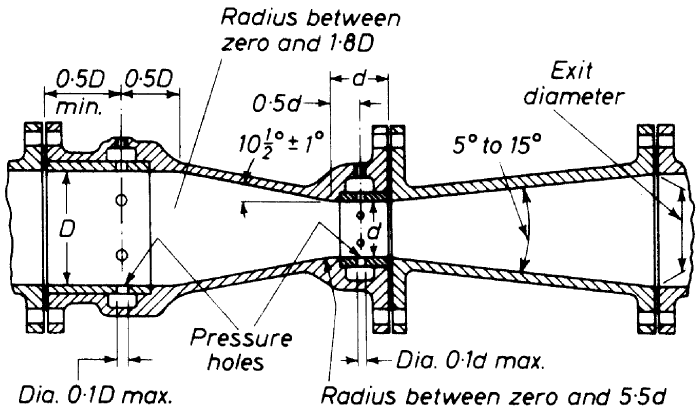
\includegraphics[width=0.5\linewidth]{FIGURES/singlevent.png}
    \caption{Single Venturi Tube~\cite{FOWLES201031}}
    \label{singlevent}
\end{figure}

The performance of a double Venturi ejector can be described using the Bernoulli equation and continuity equation, shown in equations~\ref{ec1} and ~\ref{ec2}, where $P_{1}$ and $P_{2}$ are the pressures at points 1 and 2, respectively, $\rho$ is the density of the fluid, $v_{1}$ and $v_{2}$ are the velocities at points 1 and 2, $g$ is the acceleration due to gravity, and $h_{1}$ and $h_{2}$ are the heights at points 1 and 2, and where  $u_i$ is the velocity component in the $i$-th direction.
\begin{equation}
    P_{1} + \frac{1}{2}\rho v_{1}^2 + \rho gh_{1} = P_{2} + \frac{1}{2}\rho v_{2}^2 + \rho gh_{2}
    \label{ec1}
\end{equation}
\begin{equation}
    \frac{\partial}{\partial x_i}(\rho u_i) = 0
    \label{ec2}
\end{equation}

Nevertheless, some other parameters are of significant interest. The flow rate ($Q$) through the Venturi can be determined using equation~\ref{Q} based on the discharge coefficient ($C_d$), which quantifies the flow efficiency of a fluid passing through an orifice or a venturi, it is the ratio between the actual flowrate and the ideal flowrate (predicted using the Bernoulli Equation);  the cross-sectional area of the throat ($A$), and the fluid density ($\rho$):

\begin{equation}
Q = C_d A \sqrt{\frac{2 \Delta P}{\rho}}
\label{Q}
\end{equation}

The entrainment ratio ($\omega$) and the area ratio ($A_r$) are also crucial in applications involving ejectors. The entrainment ratio is calculated using equation~\ref{entre}:

\begin{equation}
\omega = \frac{\dot{m}_s}{\dot{m}_p}
\label{entre}
\end{equation}

Where $\dot{m}_s$ is the mass flow rate of the secondary fluid and $\dot{m}_p$ is the mass flow rate of the primary fluid. The area ratio is given by equation~\ref{arearat}:

\begin{equation}
A_r = \frac{A_t}{A_e}
\label{arearat}
\end{equation}

Where $A_t$ is the throat area and $A_e$ is the exit area. 

The double Venturi configuration ensures the low-pressure zone is more pronounced, increasing the overall vacuum efficiency. Moreover, it effectively transports pollutants and particles out of piping systems~\cite{Xu2016, xiong2005three}. Figure~\ref{venturi} shows the proposed design.

\begin{figure}[H]
\centering
  \begin{subfigure}{0.5\textwidth}
  \centering
  %\hspace{-2cm}
    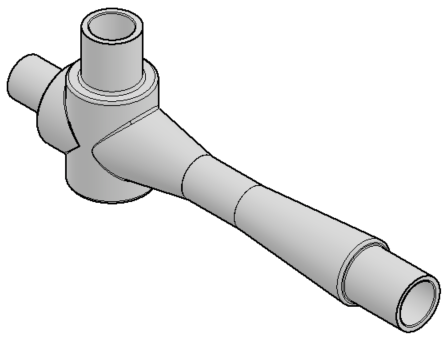
\includegraphics[width=1\linewidth]{FIGURES/venturi1.png}
    \caption{Isometric View}
  \end{subfigure}
  %\hspace{-3cm}
  \begin{subfigure}{0.5\textwidth}
  \hspace{-3cm}
    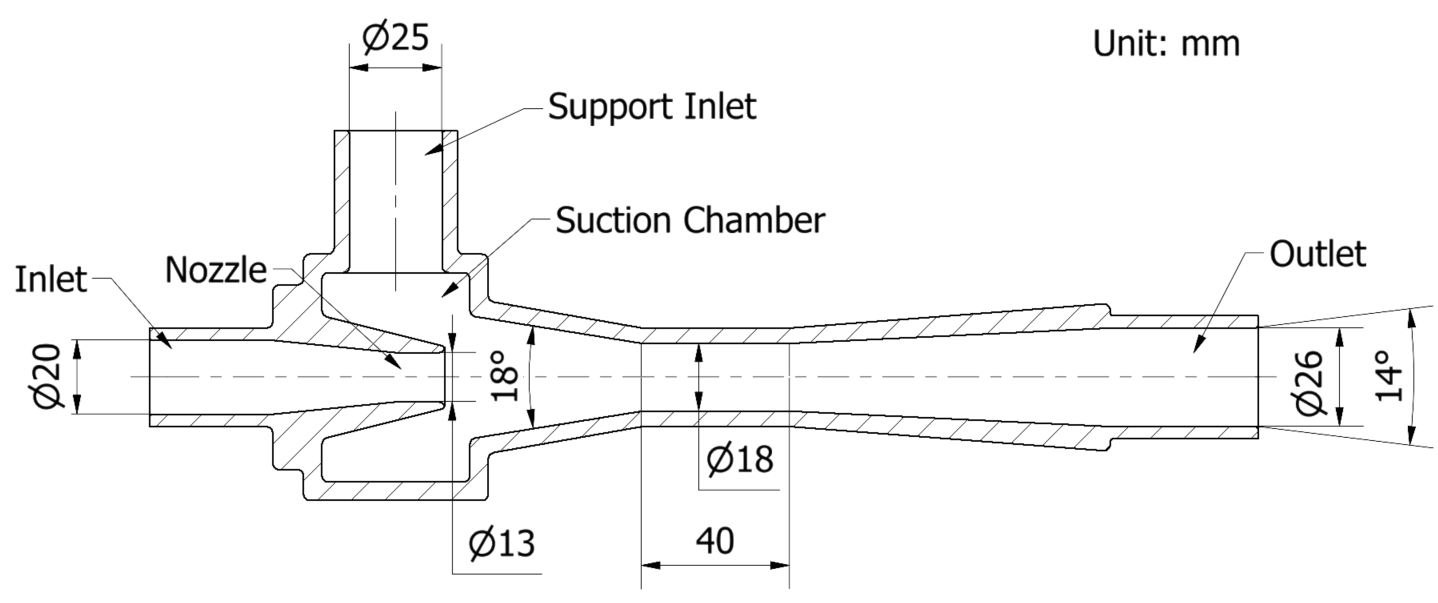
\includegraphics[width=1.7\linewidth]{FIGURES/venturi2.png}
    \caption{Half Section View}
  \end{subfigure}
  \caption{Double Venturi Ejector Structure~[Auhtor].}
    \label{venturi}
\end{figure}